% cd /disks/PROJECT/Mickael/COMMUNICATION/CST2016/;
% pdflatex THESE_CST2016_annex.tex; bibtex THESE_CST2016_annex; pdflatex THESE_CST2016_annex.tex; pdflatex THESE_CST2016_annex.tex;
% evince THESE_CST2016_annex.pdf &

\documentclass[11pt, a4paper]{article}
\documentclass[11pt, a4paper]{article}
\pdfpageattr{/Group << /S /Transparency /I true /CS /DeviceRGB>>}

\usepackage[T1]{fontenc}
\usepackage[utf8]{inputenc}
\usepackage{graphicx}
\usepackage[usenames, dvipsnames, svgnames, x11names, hyperref, RGB]{xcolor}
\usepackage{tabularx}
\usepackage{multirow}
\usepackage{pifont}
\usepackage{multicol}
\usepackage{setspace}
\renewcommand{\baselinestretch}{1.5}
\usepackage{helvet}
\renewcommand{\familydefault}{\sfdefault}

\usepackage{longtable}
\usepackage[format=plain, font=normalsize, labelfont=bf, hang]{caption}
\usepackage[hmargin=2.5cm, vmargin=2.5cm]{geometry}
\usepackage{amsmath}
\usepackage{indentfirst} % add indent in first paragraph


\usepackage{fancyhdr}
\pagestyle{fancy}
\fancyhead[L]{\slshape \rightmark}
% \fancyhead[R]{\slshape \leftmark}
% \fancyhead[L]{\today}

\usepackage{helvet}
\renewcommand{\familydefault}{\sfdefault}

\definecolor{dodgerblue}{RGB}{30,144,255}
\definecolor{springgreen3}{RGB}{0,139,69}
% \definecolor{springgreen2}{RGB}{0,205,102}
\definecolor{firebrick2}{RGB}{238,44,44}
\definecolor{maroon2}{RGB}{238,48,167}
\definecolor{goldenrod2}{RGB}{238,180,34}
\definecolor{deepskyblue}{RGB}{0,191,255}

\usepackage{textcomp}
\usepackage{listings}
\usepackage{courier}
\lstset{ %
    backgroundcolor=\color{dodgerblue!2.5!white},       % choose the background color; you must add \usepackage{color} or \usepackage{xcolor}
    basicstyle={\tiny\ttfamily\mdseries},               % the size of the fonts that are used for the code
    breakatwhitespace=true,                             % sets if automatic breaks should only happen at whitespace
    breaklines=true,                                    % sets automatic line breaking
    captionpos=t,                                       % sets the caption-position to bottom
    commentstyle=\color{springgreen3},                  % comment style
    deletekeywords={...},                               % if you want to delete keywords from the given language
    escapeinside={!*}{*!},                              % if you want to add LaTeX within your code
    extendedchars=true,                                 % lets you use non-ASCII characters; for 8-bits encodings only, does not work with UTF-8
    frame=single,                                       % adds a frame around the code
    keepspaces=true,                                    % keeps spaces in text, useful for keeping indentation of code (possibly needs columns=flexible)
    keywordstyle={\color{dodgerblue}\textbf},           % keyword style
    morekeywords={*,...},                               % if you want to add more keywords to the set
    numbers=none,                                       % where to put the line-numbers; possible values are (none, left, right)
    numbersep=10pt,                                     % how far the line-numbers are from the code
    numberstyle=\tiny\color{goldenrod2},                % the style that is used for the line-numbers
    rulecolor=\color{dodgerblue},                       % if not set, the frame-color may be changed on line-breaks within not-black text (e.g. comments (green here))
    showspaces=false,                                   % show spaces everywhere adding particular underscores; it overrides 'showstringspaces'
    showstringspaces=false,                             % underline spaces within strings only
    showtabs=false,                                     % show tabs within strings adding particular underscores
    stepnumber=1,                                       % the step between two line-numbers. If it's 1, each line will be numbered
    stringstyle=\color{maroon2},                        % string literal style
    tabsize=2,                                          % sets default tabsize to 2 spaces
    title=\lstname,                                     % show the filename of files included with \lstinputlisting; also try caption instead of title
    showlines=false,                                    % prints empty lines at the end of listings
    xleftmargin=9mm,                                    % The dimensions are used as extra margins on the left and right
    xrightmargin=9mm,
    upquote=true,
    lineskip=-0.05ex,                                   % Specifies additional space between lines in listings
    aboveskip=0ex,                                      % Define the space above and below displayed listings
    belowskip=0ex,                                      % Define the space above and below displayed listings
}
\lstdefinelanguage{JuliaConsole}{
    backgroundcolor=\color{gray!2.5!white},             % choose the background color; you must add \usepackage{color} or \usepackage{xcolor}
    rulecolor=\color{gray!50!white},                    % if not set, the frame-color may be changed on line-breaks within not-black text (e.g. comments (green here))
    alsoletter={>},
    literate=%
    *{\$}{{{\color{black}\bfseries \$}}}1
    {julia>}{{{\color{black}\bfseries julia>}}}6
}
\lstdefinelanguage{Julia}{
    keywordsprefix=\@,
    morekeywords={
        exit, whos, edit, load, is, isa, isequal, typeof, tuple, ntuple, uid, hash, finalizer, convert, promote,
        subtype, typemin, typemax, realmin, realmax, sizeof, eps, promote_type, method_exists, applicable,
        invoke, dlopen, dlsym, system, error, throw, assert, new, Inf, Nan, pi, im, begin, while, for, in, return,
        break, continue, macro, quote, let, if, elseif, else, try, catch, end, bitstype, ccall, do, using, module,
        import, export, importall, baremodule, immutable, local, global, const, Bool, Int, Int8, Int16, Int32,
        Int64, Uint, Uint8, Uint16, Uint32, Uint64, Float32, Float64, Complex64, Complex128, Any, Nothing, None,
        function, type, typealias, abstract, include, require
    },
    alsoletter={>},
    sensitive=true,
    morecomment=[l]{\#},
    morecomment=[s]{\#=}{=\#},
    morestring=[b]',
    morestring=[b]",
    literate=%
    *{0}{{{\color{goldenrod2}\textbf{0}}}}1
    {1}{{{\color{goldenrod2}\textbf{1}}}}1
    {2}{{{\color{goldenrod2}\textbf{2}}}}1
    {3}{{{\color{goldenrod2}\textbf{3}}}}1
    {4}{{{\color{goldenrod2}\textbf{4}}}}1
    {5}{{{\color{goldenrod2}\textbf{5}}}}1
    {6}{{{\color{goldenrod2}\textbf{6}}}}1
    {7}{{{\color{goldenrod2}\textbf{7}}}}1
    {8}{{{\color{goldenrod2}\textbf{8}}}}1
    {9}{{{\color{goldenrod2}\textbf{9}}}}1
    {0.0}{{{\color{goldenrod2}\textbf{0.0}}}}3
    {1.0}{{{\color{goldenrod2}\textbf{1.0}}}}3
    {2.0}{{{\color{goldenrod2}\textbf{2.0}}}}3
    {3.0}{{{\color{goldenrod2}\textbf{3.0}}}}3
    {4.0}{{{\color{goldenrod2}\textbf{4.0}}}}3
    {5.0}{{{\color{goldenrod2}\textbf{5.0}}}}3
    {6.0}{{{\color{goldenrod2}\textbf{6.0}}}}3
    {7.0}{{{\color{goldenrod2}\textbf{7.0}}}}3
    {8.0}{{{\color{goldenrod2}\textbf{8.0}}}}3
    {9.0}{{{\color{goldenrod2}\textbf{9.0}}}}3
    {0.1}{{{\color{goldenrod2}\textbf{0.1}}}}3
    {1.1}{{{\color{goldenrod2}\textbf{1.1}}}}3
    {2.1}{{{\color{goldenrod2}\textbf{2.1}}}}3
    {3.1}{{{\color{goldenrod2}\textbf{3.1}}}}3
    {4.1}{{{\color{goldenrod2}\textbf{4.1}}}}3
    {5.1}{{{\color{goldenrod2}\textbf{5.1}}}}3
    {6.1}{{{\color{goldenrod2}\textbf{6.1}}}}3
    {7.1}{{{\color{goldenrod2}\textbf{7.1}}}}3
    {8.1}{{{\color{goldenrod2}\textbf{8.1}}}}3
    {9.1}{{{\color{goldenrod2}\textbf{9.1}}}}3
    {0.2}{{{\color{goldenrod2}\textbf{0.2}}}}3
    {1.2}{{{\color{goldenrod2}\textbf{1.2}}}}3
    {2.2}{{{\color{goldenrod2}\textbf{2.2}}}}3
    {3.2}{{{\color{goldenrod2}\textbf{3.2}}}}3
    {4.2}{{{\color{goldenrod2}\textbf{4.2}}}}3
    {5.2}{{{\color{goldenrod2}\textbf{5.2}}}}3
    {6.2}{{{\color{goldenrod2}\textbf{6.2}}}}3
    {7.2}{{{\color{goldenrod2}\textbf{7.2}}}}3
    {8.2}{{{\color{goldenrod2}\textbf{8.2}}}}3
    {9.2}{{{\color{goldenrod2}\textbf{9.2}}}}3
    {0.3}{{{\color{goldenrod2}\textbf{0.3}}}}3
    {1.3}{{{\color{goldenrod2}\textbf{1.3}}}}3
    {2.3}{{{\color{goldenrod2}\textbf{2.3}}}}3
    {3.3}{{{\color{goldenrod2}\textbf{3.3}}}}3
    {4.3}{{{\color{goldenrod2}\textbf{4.3}}}}3
    {5.3}{{{\color{goldenrod2}\textbf{5.3}}}}3
    {6.3}{{{\color{goldenrod2}\textbf{6.3}}}}3
    {7.3}{{{\color{goldenrod2}\textbf{7.3}}}}3
    {8.3}{{{\color{goldenrod2}\textbf{8.3}}}}3
    {9.3}{{{\color{goldenrod2}\textbf{9.3}}}}3
    {0.4}{{{\color{goldenrod2}\textbf{0.4}}}}3
    {1.4}{{{\color{goldenrod2}\textbf{1.4}}}}3
    {2.4}{{{\color{goldenrod2}\textbf{2.4}}}}3
    {3.4}{{{\color{goldenrod2}\textbf{3.4}}}}3
    {4.4}{{{\color{goldenrod2}\textbf{4.4}}}}3
    {5.4}{{{\color{goldenrod2}\textbf{5.4}}}}3
    {6.4}{{{\color{goldenrod2}\textbf{6.4}}}}3
    {7.4}{{{\color{goldenrod2}\textbf{7.4}}}}3
    {8.4}{{{\color{goldenrod2}\textbf{8.4}}}}3
    {9.4}{{{\color{goldenrod2}\textbf{9.4}}}}3
    {0.5}{{{\color{goldenrod2}\textbf{0.5}}}}3
    {1.5}{{{\color{goldenrod2}\textbf{1.5}}}}3
    {2.5}{{{\color{goldenrod2}\textbf{2.5}}}}3
    {3.5}{{{\color{goldenrod2}\textbf{3.5}}}}3
    {4.5}{{{\color{goldenrod2}\textbf{4.5}}}}3
    {5.5}{{{\color{goldenrod2}\textbf{5.5}}}}3
    {6.5}{{{\color{goldenrod2}\textbf{6.5}}}}3
    {7.5}{{{\color{goldenrod2}\textbf{7.5}}}}3
    {8.5}{{{\color{goldenrod2}\textbf{8.5}}}}3
    {9.5}{{{\color{goldenrod2}\textbf{9.5}}}}3
    {0.6}{{{\color{goldenrod2}\textbf{0.6}}}}3
    {1.6}{{{\color{goldenrod2}\textbf{1.6}}}}3
    {2.6}{{{\color{goldenrod2}\textbf{2.6}}}}3
    {3.6}{{{\color{goldenrod2}\textbf{3.6}}}}3
    {4.6}{{{\color{goldenrod2}\textbf{4.6}}}}3
    {5.6}{{{\color{goldenrod2}\textbf{5.6}}}}3
    {6.6}{{{\color{goldenrod2}\textbf{6.6}}}}3
    {7.6}{{{\color{goldenrod2}\textbf{7.6}}}}3
    {8.6}{{{\color{goldenrod2}\textbf{8.6}}}}3
    {9.6}{{{\color{goldenrod2}\textbf{9.6}}}}3
    {0.7}{{{\color{goldenrod2}\textbf{0.7}}}}3
    {1.7}{{{\color{goldenrod2}\textbf{1.7}}}}3
    {2.7}{{{\color{goldenrod2}\textbf{2.7}}}}3
    {3.7}{{{\color{goldenrod2}\textbf{3.7}}}}3
    {4.7}{{{\color{goldenrod2}\textbf{4.7}}}}3
    {5.7}{{{\color{goldenrod2}\textbf{5.7}}}}3
    {6.7}{{{\color{goldenrod2}\textbf{6.7}}}}3
    {7.7}{{{\color{goldenrod2}\textbf{7.7}}}}3
    {8.7}{{{\color{goldenrod2}\textbf{8.7}}}}3
    {9.7}{{{\color{goldenrod2}\textbf{9.7}}}}3
    {0.8}{{{\color{goldenrod2}\textbf{0.8}}}}3
    {1.8}{{{\color{goldenrod2}\textbf{1.8}}}}3
    {2.8}{{{\color{goldenrod2}\textbf{2.8}}}}3
    {3.8}{{{\color{goldenrod2}\textbf{3.8}}}}3
    {4.8}{{{\color{goldenrod2}\textbf{4.8}}}}3
    {5.8}{{{\color{goldenrod2}\textbf{5.8}}}}3
    {6.8}{{{\color{goldenrod2}\textbf{6.8}}}}3
    {7.8}{{{\color{goldenrod2}\textbf{7.8}}}}3
    {8.8}{{{\color{goldenrod2}\textbf{8.8}}}}3
    {9.8}{{{\color{goldenrod2}\textbf{9.8}}}}3
    {0.9}{{{\color{goldenrod2}\textbf{0.9}}}}3
    {1.9}{{{\color{goldenrod2}\textbf{1.9}}}}3
    {2.9}{{{\color{goldenrod2}\textbf{2.9}}}}3
    {3.9}{{{\color{goldenrod2}\textbf{3.9}}}}3
    {4.9}{{{\color{goldenrod2}\textbf{4.9}}}}3
    {5.9}{{{\color{goldenrod2}\textbf{5.9}}}}3
    {6.9}{{{\color{goldenrod2}\textbf{6.9}}}}3
    {7.9}{{{\color{goldenrod2}\textbf{7.9}}}}3
    {8.9}{{{\color{goldenrod2}\textbf{8.9}}}}3
    {9.9}{{{\color{goldenrod2}\textbf{9.9}}}}3
    {Inf}{{{\color{goldenrod2}\textbf{Inf}}}}3
    {+}{{{\color{deepskyblue!85!black}\textbf{+}}}}1
    {-}{{{\color{deepskyblue!85!black}\textbf{-}}}}1
    {*}{{{\color{deepskyblue!85!black}\textbf{*}}}}1
    {/}{{{\color{deepskyblue!85!black}\textbf{/}}}}1
    {\%>\%}{{{\color{deepskyblue!85!black}\textbf{\%>\%}}}}3
    {R>}{{{\color{black}\bfseries R>}}}2
    {<-}{{{\color{black}\bfseries <-}}}2
    {(}{{{\color{deepskyblue!85!black}\textbf{(}}}}1
    {)}{{{\color{deepskyblue!85!black}\textbf{)}}}}1
    {[}{{{\color{deepskyblue!85!black}\textbf{[}}}}1
    {]}{{{\color{deepskyblue!85!black}\textbf{]}}}}1
    {\{}{{{\color{deepskyblue!85!black}\textbf{\{}}}}1
    {\}}{{{\color{deepskyblue!85!black}\textbf{\}}}}}1
    {julia>}{{{\color{black}\bfseries julia>}}}6
}
\lstdefinelanguage{R}{
    backgroundcolor=\color{dodgerblue!2.5!white},       % choose the background color; you must add \usepackage{color} or \usepackage{xcolor}
    rulecolor=\color{dodgerblue!50!white},              % if not set, the frame-color may be changed on line-breaks within not-black text (e.g. comments (green here))
    commentstyle=\color{springgreen3},                  % comment style
    keywordstyle={\color{dodgerblue}\textbf},           % keyword style
    numberstyle=\scriptsize\color{goldenrod2},          % the style that is used for the line-numbers
    stringstyle=\color{maroon2},                        % string literal style
    morekeywords={
        if, else, repeat, while, function, for, in, next, break, TRUE, FALSE, NULL, NA, NaN, abbreviate, abline, abs, acf, acos, acosh, addmargins, aggregate, agrep,
        alarm, alias, alist, all, anova, any, aov, aperm, append, apply, approx, approxfun, apropos, ar, args, arima, array, arrows, asin, asinh, assign, assocplot, atan,
        atanh, attach, attr, attributes, autoload, autoloader, ave, axis, backsolve, barplot, basename, beta, bindtextdomain, binomial, biplot, bitmap, bmp, body, box,
        boxplot, bquote, break, browser, builtins, bxp, by, bzfile, c call, cancor, capabilities, casefold, cat, category, cbind, ccf, ceiling, character, charmatch,
        chartr, chol, choose, chull, citation, class, close, cm, cmdscale, codes, coef, coefficients, col, colnames, colors, colorspaces, colours, comment, complex,
        confint, conflicts, contour, contrasts, contributors, convolve, cophenetic, coplot, cor, cos, cosh, cov, covratio, cpgram, crossprod, cummax, cummin, cumprod,
        cumsum, curve, cut, cutree, cycle, data, dataentry, date, dbeta, dbinom, dcauchy, dchisq, de, debug, debugger, decompose, delay, deltat, demo, dendrapply,
        density, deparse, deriv, det, detach, determinant, deviance, dexp, df, dfbeta, dfbetas, dffits, dgamma, dgeom, dget, dhyper, diag, diff, diffinv, difftime,
        digamma, dim, dimnames, dir, dirname, dist, dlnorm, dlogis, dmultinom, dnbinom, dnorm, dotchart, double, dpois, dput, drop, dsignrank, dt, dump, dunif, duplicated,
        dweibull, dwilcox, eapply, ecdf, edit, effects, eigen, emacs, embed, end, environment, eval, evalq, example, exists, exp, expression, factanal, factor, factorial,
        family, fft, fifo, file, filter, find, fitted, fivenum, fix, floor, flush, for, force, formals, format, formula, forwardsolve, fourfoldplot, frame, frequency,
        ftable, function, gamma, gaussian, gc, gcinfo, gctorture, get, getenv, geterrmessage, gettext, gettextf, getwd, gl, glm, globalenv, gray, grep, grey, grid, gsub,
        gzcon, gzfile, hat, hatvalues, hcl, hclust, head, heatmap, help, hist, history, hsv, httpclient, iconv, iconvlist, identical, identify, if, ifelse, image,
        influence, inherits, integer, integrate, interaction, interactive, intersect, invisible, isoreg, jitter, jpeg, julian, kappa, kernapply, kernel, kmeans, knots,
        kronecker, ksmooth, labels, lag, lapply, layout, lbeta, lchoose, lcm, legend, length, letters, levels, lfactorial, lgamma, library, licence, license, line, lines,
        list, lm, load, loadhistory, loadings, local, locator, loess, log, logb, logical, loglin, lowess, ls, lsfit, machine, mad, mahalanobis, makepredictcall, manova,
        mapply, match, matlines, matplot, matpoints, matrix, max, mean, median, medpolish, menu, merge, message, methods, mget, min, missing, mode, monthplot, months,
        mosaicplot, mtext, mvfft, names, napredict, naprint, naresid, nargs, nchar, ncol, next, nextn, ngettext, nlevels, nlm, nls, noquote, nrow, numeric, objects, offset,
        open, optim, optimise, optimize, options, order, ordered, outer, pacf, page, pairlist, pairs, palette, par, parse, paste, pbeta, pbinom, pbirthday, pcauchy, pchisq,
        pdf, pentagamma, person, persp, pexp, pf, pgamma, pgeom, phyper, pi, pico, pictex, pie, piechart, pipe, plclust, plnorm, plogis, plot, pmatch, pmax, pmin, pnbinom,
        png, pnorm, points, poisson, poly, polygon, polym, polyroot, postscript, power, ppoints, ppois, ppr, prcomp, predict, preplot, pretty, princomp, print, prmatrix,
        prod, profile, profiler, proj, promax, prompt, provide, psigamma, psignrank, pt, ptukey, punif, pweibull, pwilcox, q qbeta, qbinom, qbirthday, qcauchy, qchisq, qexp,
        qf, qgamma, qgeom, qhyper, qlnorm, qlogis, qnbinom, qnorm, qpois, qqline, qqnorm, qqplot, qr, qsignrank, qt, qtukey, quantile, quarters, quasi, quasibinomial,
        quasipoisson, quit, qunif, quote, qweibull, qwilcox, rainbow, range, rank, raw, rbeta, rbind, rbinom, rcauchy, rchisq, readline, real, recover, rect, reformulate,
        regexpr, relevel, remove, reorder, rep, repeat, replace, replicate, replications, require, reshape, resid, residuals, restart, return, rev, rexp, rf, rgamma, rgb,
        rgeom, rhyper, rle, rlnorm, rlogis, rm, rmultinom, rnbinom, rnorm, round, row, rownames, rowsum, rpois, rsignrank, rstandard, rstudent, rt, rug, runif, runmed,
        rweibull, rwilcox, sample, sapply, save, savehistory, scale, scan, screen, screeplot, sd, search, searchpaths, seek, segments, seq, sequence, serialize, setdiff,
        setequal, setwd, shell, sign, signif, sin, single, sinh, sink, smooth, solve, sort, source, spectrum, spline, splinefun, split, sprintf, sqrt, stack, stars, start,
        stderr, stdin, stdout, stem, step, stepfun, stl, stop, stopifnot, str, strftime, strheight, stripchart, strptime, strsplit, strtrim, structure, strwidth, strwrap,
        sub, subset, substitute, substr, substring, sum, summary, sunflowerplot, supsmu, svd, sweep, switch, symbols, symnum, system, t table, tabulate, tail, tan, tanh,
        tapply, tempdir, tempfile, termplot, terms, tetragamma, text, time, title, toeplitz, tolower, topenv, toupper, trace, traceback, transform, trigamma, trunc,
        truncate, try, ts, tsdiag, tsp, typeof, unclass, undebug, union, unique, uniroot, unix, unlink, unlist, unname, unserialize, unsplit, unstack, untrace, unz,
        update, upgrade, url, var, varimax, vcov, vector, version, vi, vignette, warning, warnings, weekdays, weights, which, while, window, windows, with, write,
        wsbrowser, xedit, xemacs, xfig, xinch, xor, xtabs, xyinch, yinch, zapsmall,
        ggplot, ggvis
    },
    sensitive=true,
    morecomment=[l]{\#},
    morestring=[b]',
    morestring=[b]",
    literate=%
    *{0}{{{\color{goldenrod2}\textbf{0}}}}1
    {1}{{{\color{goldenrod2}\textbf{1}}}}1
    {2}{{{\color{goldenrod2}\textbf{2}}}}1
    {3}{{{\color{goldenrod2}\textbf{3}}}}1
    {4}{{{\color{goldenrod2}\textbf{4}}}}1
    {5}{{{\color{goldenrod2}\textbf{5}}}}1
    {6}{{{\color{goldenrod2}\textbf{6}}}}1
    {7}{{{\color{goldenrod2}\textbf{7}}}}1
    {8}{{{\color{goldenrod2}\textbf{8}}}}1
    {9}{{{\color{goldenrod2}\textbf{9}}}}1
    {0.0}{{{\color{goldenrod2}\textbf{0.0}}}}3
    {1.0}{{{\color{goldenrod2}\textbf{1.0}}}}3
    {2.0}{{{\color{goldenrod2}\textbf{2.0}}}}3
    {3.0}{{{\color{goldenrod2}\textbf{3.0}}}}3
    {4.0}{{{\color{goldenrod2}\textbf{4.0}}}}3
    {5.0}{{{\color{goldenrod2}\textbf{5.0}}}}3
    {6.0}{{{\color{goldenrod2}\textbf{6.0}}}}3
    {7.0}{{{\color{goldenrod2}\textbf{7.0}}}}3
    {8.0}{{{\color{goldenrod2}\textbf{8.0}}}}3
    {9.0}{{{\color{goldenrod2}\textbf{9.0}}}}3
    {0.1}{{{\color{goldenrod2}\textbf{0.1}}}}3
    {1.1}{{{\color{goldenrod2}\textbf{1.1}}}}3
    {2.1}{{{\color{goldenrod2}\textbf{2.1}}}}3
    {3.1}{{{\color{goldenrod2}\textbf{3.1}}}}3
    {4.1}{{{\color{goldenrod2}\textbf{4.1}}}}3
    {5.1}{{{\color{goldenrod2}\textbf{5.1}}}}3
    {6.1}{{{\color{goldenrod2}\textbf{6.1}}}}3
    {7.1}{{{\color{goldenrod2}\textbf{7.1}}}}3
    {8.1}{{{\color{goldenrod2}\textbf{8.1}}}}3
    {9.1}{{{\color{goldenrod2}\textbf{9.1}}}}3
    {0.2}{{{\color{goldenrod2}\textbf{0.2}}}}3
    {1.2}{{{\color{goldenrod2}\textbf{1.2}}}}3
    {2.2}{{{\color{goldenrod2}\textbf{2.2}}}}3
    {3.2}{{{\color{goldenrod2}\textbf{3.2}}}}3
    {4.2}{{{\color{goldenrod2}\textbf{4.2}}}}3
    {5.2}{{{\color{goldenrod2}\textbf{5.2}}}}3
    {6.2}{{{\color{goldenrod2}\textbf{6.2}}}}3
    {7.2}{{{\color{goldenrod2}\textbf{7.2}}}}3
    {8.2}{{{\color{goldenrod2}\textbf{8.2}}}}3
    {9.2}{{{\color{goldenrod2}\textbf{9.2}}}}3
    {0.3}{{{\color{goldenrod2}\textbf{0.3}}}}3
    {1.3}{{{\color{goldenrod2}\textbf{1.3}}}}3
    {2.3}{{{\color{goldenrod2}\textbf{2.3}}}}3
    {3.3}{{{\color{goldenrod2}\textbf{3.3}}}}3
    {4.3}{{{\color{goldenrod2}\textbf{4.3}}}}3
    {5.3}{{{\color{goldenrod2}\textbf{5.3}}}}3
    {6.3}{{{\color{goldenrod2}\textbf{6.3}}}}3
    {7.3}{{{\color{goldenrod2}\textbf{7.3}}}}3
    {8.3}{{{\color{goldenrod2}\textbf{8.3}}}}3
    {9.3}{{{\color{goldenrod2}\textbf{9.3}}}}3
    {0.4}{{{\color{goldenrod2}\textbf{0.4}}}}3
    {1.4}{{{\color{goldenrod2}\textbf{1.4}}}}3
    {2.4}{{{\color{goldenrod2}\textbf{2.4}}}}3
    {3.4}{{{\color{goldenrod2}\textbf{3.4}}}}3
    {4.4}{{{\color{goldenrod2}\textbf{4.4}}}}3
    {5.4}{{{\color{goldenrod2}\textbf{5.4}}}}3
    {6.4}{{{\color{goldenrod2}\textbf{6.4}}}}3
    {7.4}{{{\color{goldenrod2}\textbf{7.4}}}}3
    {8.4}{{{\color{goldenrod2}\textbf{8.4}}}}3
    {9.4}{{{\color{goldenrod2}\textbf{9.4}}}}3
    {0.5}{{{\color{goldenrod2}\textbf{0.5}}}}3
    {1.5}{{{\color{goldenrod2}\textbf{1.5}}}}3
    {2.5}{{{\color{goldenrod2}\textbf{2.5}}}}3
    {3.5}{{{\color{goldenrod2}\textbf{3.5}}}}3
    {4.5}{{{\color{goldenrod2}\textbf{4.5}}}}3
    {5.5}{{{\color{goldenrod2}\textbf{5.5}}}}3
    {6.5}{{{\color{goldenrod2}\textbf{6.5}}}}3
    {7.5}{{{\color{goldenrod2}\textbf{7.5}}}}3
    {8.5}{{{\color{goldenrod2}\textbf{8.5}}}}3
    {9.5}{{{\color{goldenrod2}\textbf{9.5}}}}3
    {0.6}{{{\color{goldenrod2}\textbf{0.6}}}}3
    {1.6}{{{\color{goldenrod2}\textbf{1.6}}}}3
    {2.6}{{{\color{goldenrod2}\textbf{2.6}}}}3
    {3.6}{{{\color{goldenrod2}\textbf{3.6}}}}3
    {4.6}{{{\color{goldenrod2}\textbf{4.6}}}}3
    {5.6}{{{\color{goldenrod2}\textbf{5.6}}}}3
    {6.6}{{{\color{goldenrod2}\textbf{6.6}}}}3
    {7.6}{{{\color{goldenrod2}\textbf{7.6}}}}3
    {8.6}{{{\color{goldenrod2}\textbf{8.6}}}}3
    {9.6}{{{\color{goldenrod2}\textbf{9.6}}}}3
    {0.7}{{{\color{goldenrod2}\textbf{0.7}}}}3
    {1.7}{{{\color{goldenrod2}\textbf{1.7}}}}3
    {2.7}{{{\color{goldenrod2}\textbf{2.7}}}}3
    {3.7}{{{\color{goldenrod2}\textbf{3.7}}}}3
    {4.7}{{{\color{goldenrod2}\textbf{4.7}}}}3
    {5.7}{{{\color{goldenrod2}\textbf{5.7}}}}3
    {6.7}{{{\color{goldenrod2}\textbf{6.7}}}}3
    {7.7}{{{\color{goldenrod2}\textbf{7.7}}}}3
    {8.7}{{{\color{goldenrod2}\textbf{8.7}}}}3
    {9.7}{{{\color{goldenrod2}\textbf{9.7}}}}3
    {0.8}{{{\color{goldenrod2}\textbf{0.8}}}}3
    {1.8}{{{\color{goldenrod2}\textbf{1.8}}}}3
    {2.8}{{{\color{goldenrod2}\textbf{2.8}}}}3
    {3.8}{{{\color{goldenrod2}\textbf{3.8}}}}3
    {4.8}{{{\color{goldenrod2}\textbf{4.8}}}}3
    {5.8}{{{\color{goldenrod2}\textbf{5.8}}}}3
    {6.8}{{{\color{goldenrod2}\textbf{6.8}}}}3
    {7.8}{{{\color{goldenrod2}\textbf{7.8}}}}3
    {8.8}{{{\color{goldenrod2}\textbf{8.8}}}}3
    {9.8}{{{\color{goldenrod2}\textbf{9.8}}}}3
    {0.9}{{{\color{goldenrod2}\textbf{0.9}}}}3
    {1.9}{{{\color{goldenrod2}\textbf{1.9}}}}3
    {2.9}{{{\color{goldenrod2}\textbf{2.9}}}}3
    {3.9}{{{\color{goldenrod2}\textbf{3.9}}}}3
    {4.9}{{{\color{goldenrod2}\textbf{4.9}}}}3
    {5.9}{{{\color{goldenrod2}\textbf{5.9}}}}3
    {6.9}{{{\color{goldenrod2}\textbf{6.9}}}}3
    {7.9}{{{\color{goldenrod2}\textbf{7.9}}}}3
    {8.9}{{{\color{goldenrod2}\textbf{8.9}}}}3
    {9.9}{{{\color{goldenrod2}\textbf{9.9}}}}3
    {Inf}{{{\color{goldenrod2}\textbf{Inf}}}}3
    {+}{{{\color{deepskyblue!85!black}\textbf{+}}}}1
    {-}{{{\color{deepskyblue!85!black}\textbf{-}}}}1
    {*}{{{\color{deepskyblue!85!black}\textbf{*}}}}1
    {/}{{{\color{deepskyblue!85!black}\textbf{/}}}}1
    {\%>\%}{{{\color{deepskyblue!85!black}\textbf{\%>\%}}}}3
    {R>}{{{\color{black}\bfseries R>}}}2
    {<-}{{{\color{black}\bfseries <-}}}2
    {(}{{{\color{deepskyblue!85!black}\textbf{(}}}}1
    {)}{{{\color{deepskyblue!85!black}\textbf{)}}}}1
    {[}{{{\color{deepskyblue!85!black}\textbf{[}}}}1
    {]}{{{\color{deepskyblue!85!black}\textbf{]}}}}1
    {\{}{{{\color{deepskyblue!85!black}\textbf{\{}}}}1
    {\}}{{{\color{deepskyblue!85!black}\textbf{\}}}}}1
}
\lstdefinelanguage{md}{
    backgroundcolor=\color{dodgerblue!2.5!white},       % choose the background color; you must add \usepackage{color} or \usepackage{xcolor}
    rulecolor=\color{dodgerblue!50!white},              % if not set, the frame-color may be changed on line-breaks within not-black text (e.g. comments (green here))
    commentstyle=\color{springgreen3},                  % comment style
    keywordstyle={\color{dodgerblue}\textbf},           % keyword style
    numberstyle=\scriptsize\color{goldenrod2},          % the style that is used for the line-numbers
    stringstyle=\color{maroon2},                        % string literal style
    morecomment=[l][\color{dodgerblue}\textbf]{\#},
    sensitive=true,
    literate=%
    {à}{{\`a}}1
    {è}{{\`e}}1
    {é}{{\'e}}1
    {ê}{{\^e}}1
    {`}{{{\color{dodgerblue}\textbf{`}}}}1
    {*}{{{\color{dodgerblue}\textbf{*}}}}1
    {(}{{{\color{deepskyblue!85!black}\textbf{(}}}}1
    {)}{{{\color{deepskyblue!85!black}\textbf{)}}}}1
    {[}{{{\color{deepskyblue!85!black}\textbf{[}}}}1
    {]}{{{\color{deepskyblue!85!black}\textbf{]}}}}1
    {\{}{{{\color{deepskyblue!85!black}\textbf{\{}}}}1
    {\}}{{{\color{deepskyblue!85!black}\textbf{\}}}}}1
}
\lstdefinelanguage{yaml}{
    morecomment=[s]{<!--}{-->},
    morekeywords={
        output, word_document, html_document, pdf_document, beamer_presentation
    }
}
\usepackage{etoolbox}
\makeatletter
\patchcmd{\lsthk@SelectCharTable}{%
  \lst@ifbreaklines\lst@Def{`)}{\lst@breakProcessOther)}\fi
}{%
}{
}{
}
\makeatother

\newif\ifblacked\blackedfalse
\ifblacked
    \usepackage[colorlinks=true,
        linkcolor=black,
        urlcolor=black,
        citecolor=black,
        filecolor=black,
        menucolor=black,
        pdftex=true,
        bookmarks=true,
        bookmarksopen=true,
        hyperfootnotes=true,
        pdfauthor={Mickaël Canouil},
        pdfcreator={Mickaël Canouil}]{hyperref}
    \renewcommand{\thefootnote}{\textcolor{black}{\arabic{footnote}}}
\else
    \usepackage[colorlinks=true,
        linkcolor=firebrick2,
        urlcolor=maroon2,
        citecolor=dodgerblue,
        filecolor=goldenrod2,
        menucolor=dodgerblue,
        pdftex=true,
        bookmarks=true,
        bookmarksopen=true,
        hyperfootnotes=true,
        pdfauthor={Mickaël Canouil},
        pdfcreator={Mickaël Canouil}]{hyperref}
    \renewcommand{\thefootnote}{\textcolor{springgreen3}{\arabic{footnote}}}
\fi

\usepackage[all]{hypcap}

\renewcommand{\baselinestretch}{1.5}

\setlength{\headheight}{15pt}
\setlength{\abovecaptionskip}{0pt}
\setlength{\tabcolsep}{10pt} % default

\newlength{\wideitemsep}
\setlength{\wideitemsep}{.5\itemsep}
\addtolength{\wideitemsep}{-7pt}
\let\olditem\item
\newcommand{\items}{\setlength{\itemsep}{\wideitemsep}\olditem}

\usepackage[square, authoryear]{natbib}
\bibliographystyle{apalike}

\makeatletter
	\def\maketitle{
        \hypersetup{pageanchor=false}
		\begin{titlepage}
			\begin{center}
				{\setlength{\baselineskip}{0.5\baselineskip}
					{\Large{\@institute}\linebreak}
				\par}
					\vskip 0cm
				{\setlength{\baselineskip}{0.5\baselineskip}
					{\small{\@address}\linebreak}
				\par}
					\vfill
                {\setlength{\baselineskip}{1.5\baselineskip}
                    {\Huge{\bf\@title}}
                \par}
					\vskip 2cm
				{\Large{\@author}}
					\vskip 0.25cm
				{\setlength{\baselineskip}{0.5\baselineskip}
					{\small{\@grade}}
				\par}
					\vskip 0cm
				{\setlength{\baselineskip}{0.5\baselineskip}
					{\footnotesize{(\@email)}}
				\par}
                    \vskip 1cm
				{\setlength{\baselineskip}{0.75\baselineskip}
					{\small{\@cst}\linebreak}
				\par}
					\vfill
				{\large{\@date}}
					\vskip 2cm
				{
\includegraphics[height=60pt, keepaspectratio]{./Logos/logo_cnrs.pdf} \hfill 
\includegraphics[height=60pt, keepaspectratio]{./Logos/UL2-WEB-2014.png} \hfill 
\includegraphics[height=60pt, keepaspectratio]{./Logos/Institut-Pasteur-de-Lille.png} \hfill 
\includegraphics[height=60pt, keepaspectratio]{./Logos/logo_egid.pdf}}
			\end{center}
		\end{titlepage}
        \hypersetup{pageanchor=true}
	}
	\def\email#1{\def\@email{#1}}
	\def\institute#1{\def\@institute{#1}}
	\def\address#1{\def\@address{#1}}
	\def\grade#1{\def\@grade{#1}}
	\def\cst#1{\def\@cst{#1}}
\makeatother


\newcommand\bref[2]{\hyperref[#1]{#2~\ref*{#1}}}
\newcommand\cmd[1]{\texttt{\color{black}\textbf{#1}}}
\newcommand\cmdb[1]{\texttt{\color{dodgerblue}\textbf{#1}}}
\newcommand\cmdr[1]{\texttt{\color{firebrick2}\textbf{#1}}}
\newcommand\cmdg[1]{\texttt{\color{springgreen3}\textbf{#1}}}
\newcommand\cmdy[1]{\texttt{\color{goldenrod2}\textbf{#1}}}
\newcommand\blue[1]{{\color{dodgerblue}\textbf{#1}}}
\newcommand\red[1]{{\color{firebrick2}\textbf{#1}}}
\newcommand\green[1]{{\color{springgreen3}\textbf{#1}}}
\newcommand\yellow[1]{{\color{goldenrod2}\textbf{#1}}}
\newcommand\pql{{\rmfamily \textbf{\color{goldenrod2}``}}}
\newcommand\pqr{{\rmfamily \textbf{\color{goldenrod2}''}}}
\newcommand\pq[3]{{\rmfamily \textbf{\color{#3}``}}#1{\rmfamily \textbf{\color{#3}''}} - \textcolor{#3}{#2}}
\newenvironment{bquote}[1]
    {\begin{quotation}
    \vspace{10pt}
    \newcommand{\bqauthor}{\normalfont \begin{quote}\begin{flushright}--- #1\end{flushright}\end{quote}}
    \rmfamily \itshape {\huge\textbf{``}}
    }
    {{\huge\textbf{''}}
    \bqauthor
    \end{quotation}
    }
\newcommand\lettrine[1]{{\huge{$\mathcal{#1}$}}}

\newcommand{\R}{\protect\includegraphics[height=0.5cm, keepaspectratio]{./Logos/logo_R.pdf}}
\newcommand{\Julia}{\protect{\raisebox{-0.5ex}{
\includegraphics[height=0.5cm, keepaspectratio]{./Logos/logo_julia.pdf}}}}

\usepackage{eso-pic}
\usepackage{transparent}
% \AddToShipoutPicture*{\AtPageLowerLeft{\transparent{0.30}
\includegraphics[width=\paperwidth,height=\paperheight]{figures/BG03_A0.jpg}}}

\usepackage{pdfpages}

\usepackage[english, francais]{babel}
\selectlanguage{francais}

\addto\captionsfrancais{%
   \def\figurename{Figure}%
}
\addto\captionsfrancais{%
   \def\tablename{Table}%
}

\title{\huge{Développement et Application de Méthodologies Statistiques pour Etudes Longitudinales d'Association Génétique}\linebreak \large{\textit{Comité de Suivi de Thèse: deuxième année}}}
\date{26 septembre 2016}
\email{\href{mailto:mickael.canouil@cnrs.fr}{mickael.canouil@cnrs.fr}}
\author{Mickaël Canouil}
\grade{Doctorant en Biostatistique}
\institute{\cmdb{G}énomique \cmdb{I}ntégrative et \cmdb{M}odélisation des \cmdb{M}aladies \cmdb{M}étaboliques \linebreak UMR 8199 (CNRS / Université de Lille 2 / Institut Pasteur de Lille)}
\address{CNRS UMR 8199 - Institut de Biologie de Lille\linebreak
1 Rue du Professeur Calmette\linebreak
BP 245\linebreak
F-59019 LILLE CEDEX
}
\cst{
\textbf{Directeur de thèse:}\\ Pr. Philippe Froguel\\ \vskip 0.25cm
\textbf{Co-directeur de thèse:}\\ Dr. Ghislain Rocheleau (Lille 2)\\ \vskip 0.25cm
\textbf{Membres du CST:}\\ Dr. Hélène Jacqmin-Gadda (INSERM U 897, Bordeaux)\\
Pr. Cristian Preda (Ecole Polytechnique, Lille)
}

% <<title, echo = FALSE, results = hide>>=
% @


\begin{document}
% \maketitle
% \tableofcontents

\clearpage
\section{Travaux précédents}
\subsection{Modèle Joint}
\begin{figure}[ht]
    \begin{center}
        \fbox{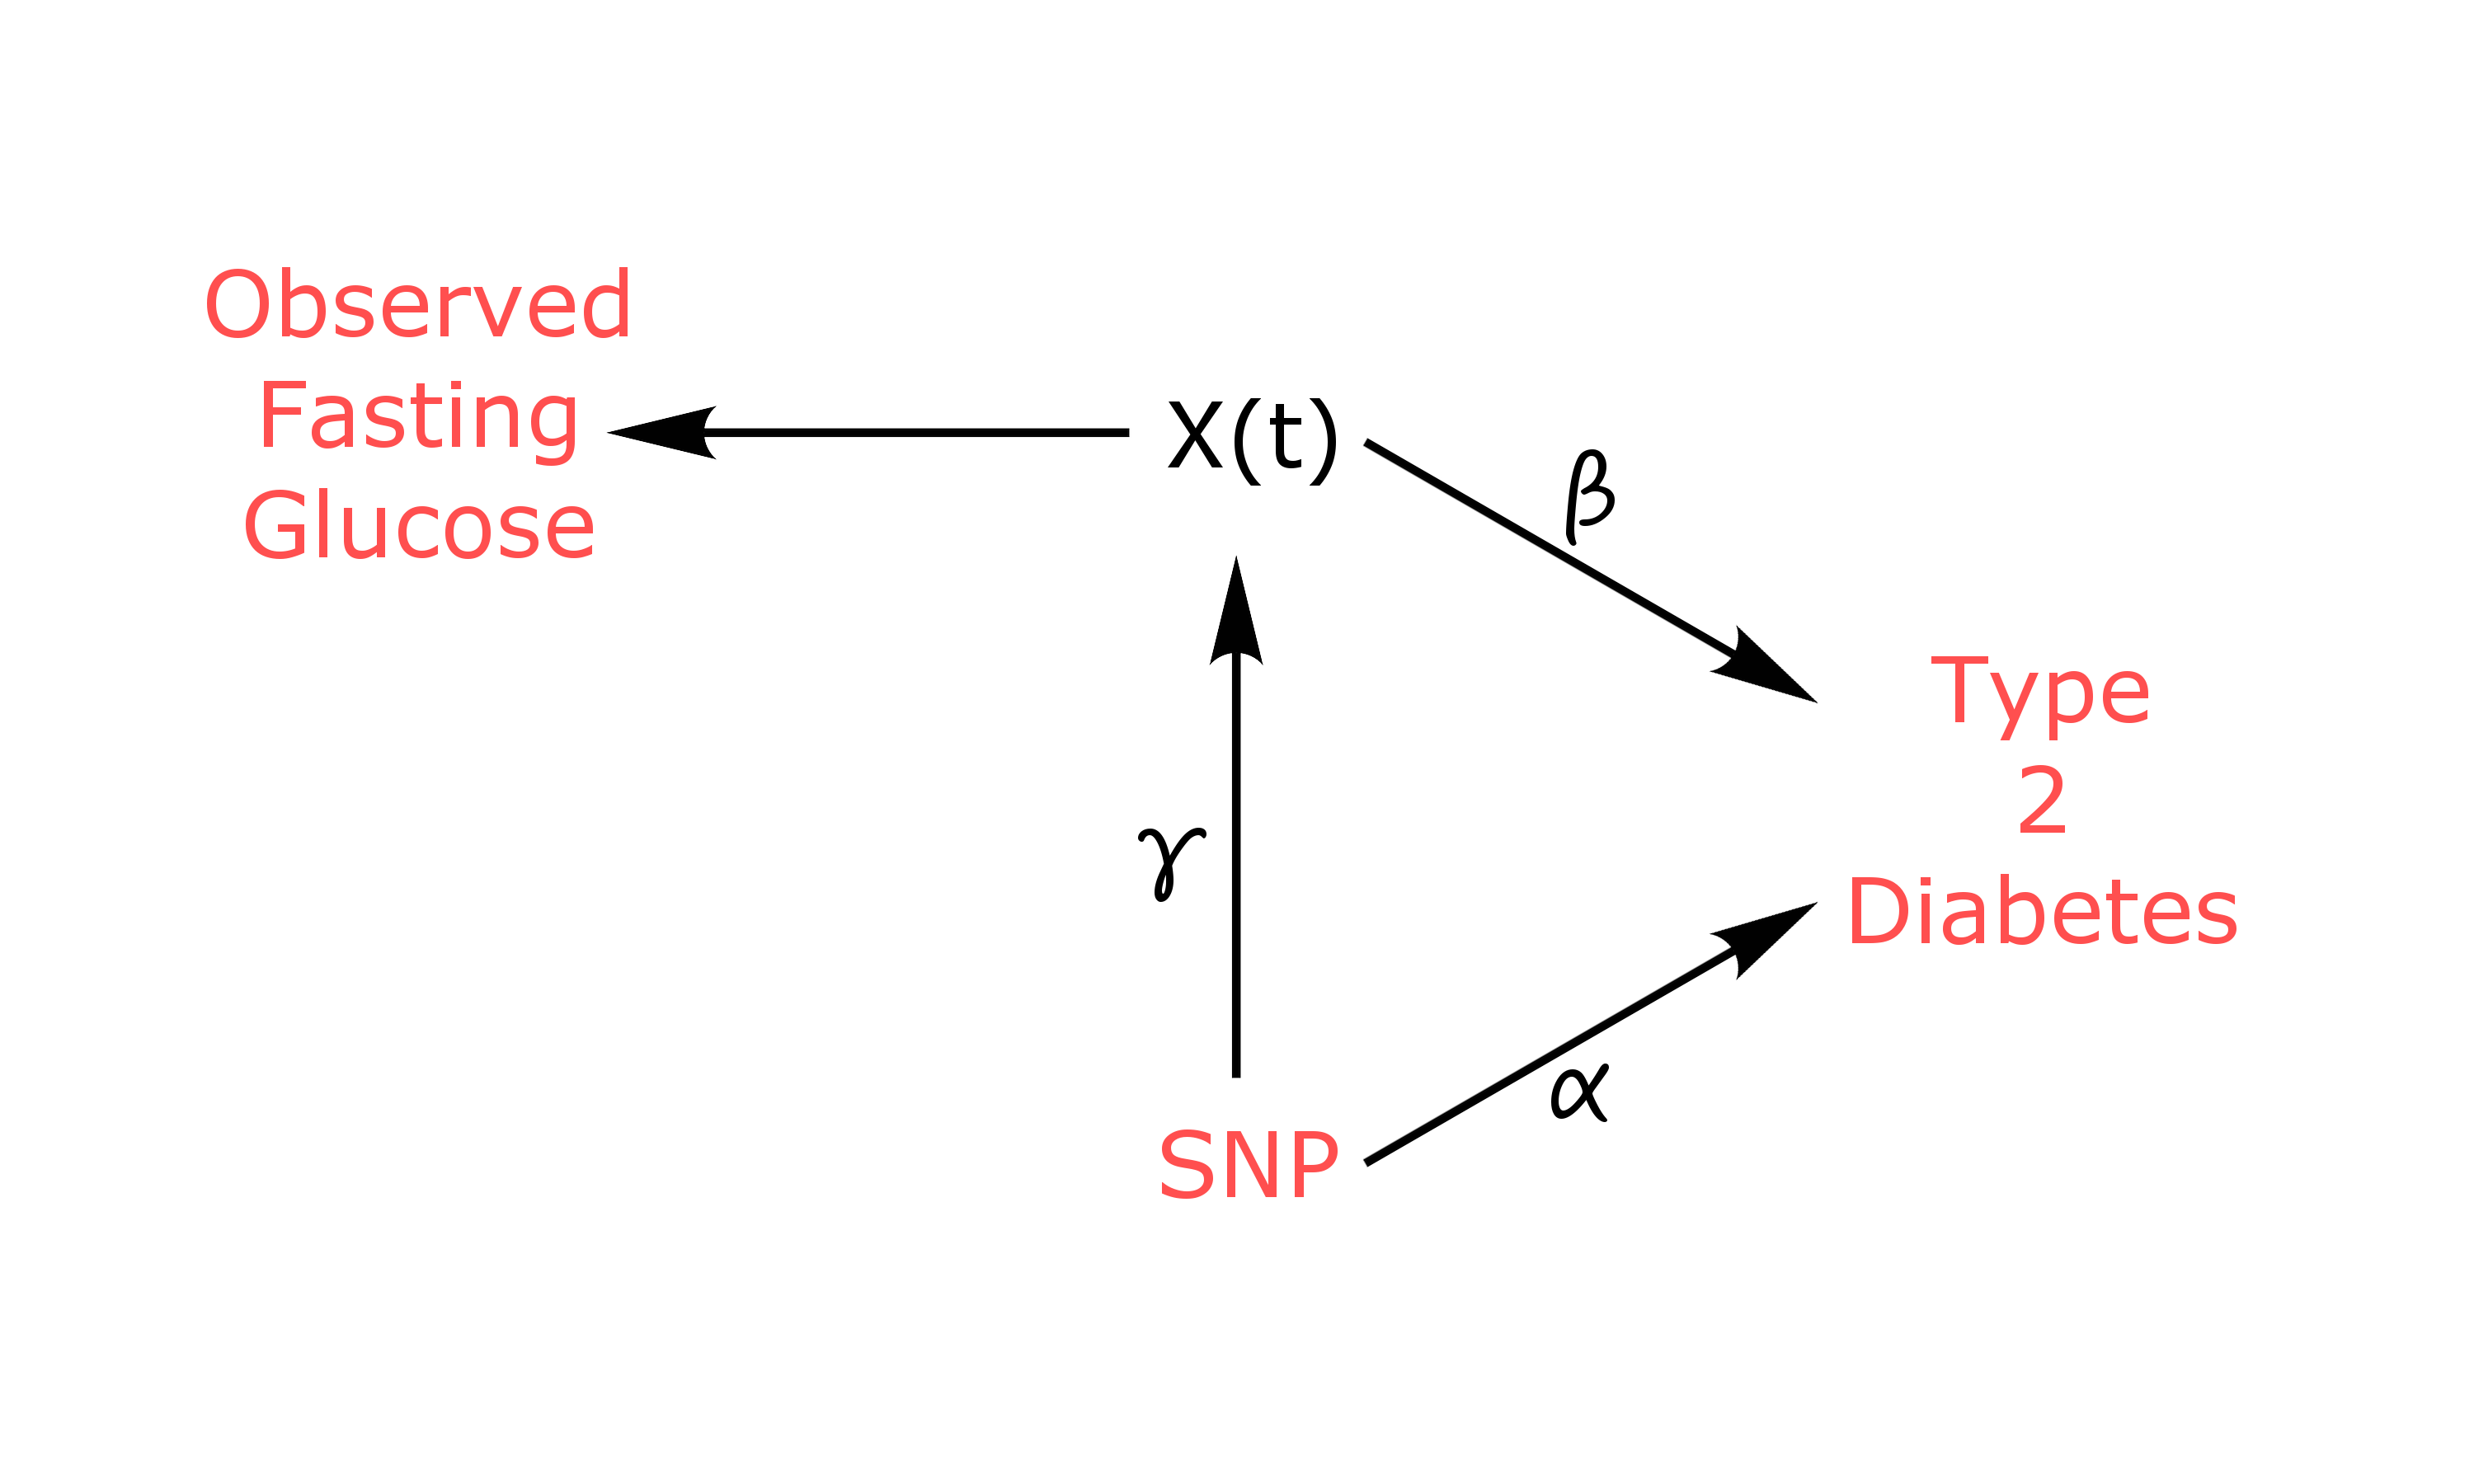
\includegraphics[width=7.5cm]{figures/jointModel.png}}
    \end{center}
    \vspace{-15pt}
    \captionof{figure}{Diagramme général d'un modèle joint pour le T2D (adapté de \cite{ibrahim_basic_2010})\newline
    {\small $X(t)$: trajectoire de la glycémie à jeun inférée des données longitudinales observées;
    $\alpha$: effet du SNP sur le diabète;
    $\gamma$: effet du SNP sur la trajectoire de la glycémie à jeun;
    $\beta$: effet de la trajectoire de la glycémie à jeun sur le diabète.}}
    \label{fig:JointModel}
\end{figure}
\par{En utilisant, l'approche de modèle joint implémentée dans l'extension JM \citep{rizopoulos_jm_2010} du logiciel R (version 3.2.3)\citep{r_core_team_r_2015},
124~095 SNPs de la MetaboChip ont été testés simultanément pour leur association avec la glycémie à jeun et le risque de DT2.}

\par{La formulation standard du modèle joint implique deux composantes, d'une part, une composante longitudinale pour modéliser la trajectoire de la variable étudiée,
et d'autre part, une composante de survie pour modéliser la survenue de l'événement étudié.
La composante longitudinale consiste typiquement à l'application d'un modèle linéaire mixte:
\begin{eqnarray}Y_{ij}=X_{ij}+\epsilon_{ij},\label{eq:1}\end{eqnarray}
où $Y_{ij}$ est la valeur observée et $X_{ij}$ la vraie (non-observée) valeur de la variable longitudinale.
Le terme $\epsilon_{ij}$ est le terme d'erreur aléatoire supposé être distribué selon la Loi Normale:
\begin{eqnarray}\epsilon_{ij} \sim \mathcal{N}(0, \sigma^2)\label{eq:2}\end{eqnarray}
La quantité $X_{ij}$ (ou $X(t)$) est la fonction de la trajectoire et est définie usuellement comme une fonction linéaire (ou quadratique) du temps $t$.}

\par{Des covariables peuvent être incluses dans la fonction de la trajectoire, comme l'âge, le sexe ou l'IMC.
Dans notre étude, $Y_{ij}$ représente les valeurs mesurées la glycémie à jeun au temps $t_{ij}$, $Z_i$ désigne le génotype du SNP analysé pour l'individu $i$ et $W_i$ désigne les covariables selon le modèle suivant:
\begin{eqnarray}Y_{ij}=X_{ij}+\epsilon_{ij}=\theta_{0i}+\theta_{1i}\times t_{ij}+\gamma \times Z_i+\delta \times W_i\epsilon_{ij}\label{eq:3}\end{eqnarray}
Pour simplifier, le terme $\delta \times W_i$ sera omis dans la suite.}

\par{Les paramètres $\theta_{0i}$ et $\theta_{1i}$ sont supposés être distribués selon une distribution normale multivariée:
\begin{eqnarray}\boldsymbol\theta \sim \mathcal{N}_2(\boldsymbol\mu, \boldsymbol\Sigma)\label{eq:4}\end{eqnarray}
Le paramètre $\gamma$ évalue l'effet additif du SNP ($Z_i$) sur la fonction de la trajectoire.
Pour tenir compte éventuellement de pentes variant entre les génotypes, un terme d'interaction entre le SNP et le temps peut être inclus dans la fonction de la trajectoire.
Le terme d'interaction n'a pas été inclus dans notre étude.}

\par{La composante de survie (survenue du DT2) se compose généralement d'un modèle paramétrique (p.ex. exponentielle ou Weibull) ou semi-paramétrique (p.ex. risques proportionnels de Cox) avec:
\begin{eqnarray}h_i(t)=h_0(t) exp(\beta X_i(t)+\alpha Z_i),\label{eq:5}\end{eqnarray}
où $h_i(t)$ est la fonction de risque au temps $t$ pour l'individu $i$ et $h_0(t)$ est la fonction de risque de base non spécifiée, supposée être une constante par morceaux avec deux noeuds placés à des temps intermédiaires
(c'est-à-dire, à trois et six ans sur les neuf ans du suivi). Le coefficient $\alpha$ mesure l'effet du SNP sur le délai d'apparition du DT2,
alors que le coefficient $\beta$ mesure l'association entre la trajectoire du niveau de la glycémie à jeun et le temps d'apparition du DT2.}

\clearpage
\subsection{Simulation}
\par{Des études de simulation ont été menées pour examiner la puissance statistique et l'erreur de type 1 des SNPs trouvés comme nominalement associé (à 5\%) en utilisant le modèle joint, comme implémenté par \citet{rizopoulos_jm_2010}.
Notre objectif principal était de déterminer le gain ou la perte de puissance du modèle joint par rapport aux approches classiques transversales (p.ex. régression logistique ou linéaire, modèle de Cox)
pour détecter l'effet d'un SNP, sur la glycémie à jeun et le statut DT2 dans notre étude.
Les jeux de données de simulation, qui ont été réalisés avec R, suivent les \hyperref[eq:1]{Equations~\ref*{eq:1}~à~\ref{eq:5}},
avec la fonction de risque de base fixée ($h_0(t)=\lambda$) de façon à obtenir une incidence équivalente à celle de la cohorte D.E.S.I.R (environ 5\%), durant la période de suivi de neuf ans.
Les temps d'événements ont été générés selon une distribution exponentielle dans le cadre du modèle de Cox à risque proportionnel \citep{austin_generating_2012}.
\begin{eqnarray}H(T)=\int_0^T \lambda exp(\beta \times X(t) + \alpha \times Z) dt\end{eqnarray}
\begin{eqnarray}T=\frac{1}{\beta\theta_1} log\left( - \frac{\beta\theta_1 \times log(1-u)}{\lambda exp(\beta\theta_0+(\beta\gamma+\alpha)Z)}+1 \right)\end{eqnarray}
}

\clearpage
\subsection{Etudes des estimateurs du modèle joint par simulation}
\begin{table}[h]
    \begin{center}
        \begin{tabular}{lc}
            \hline
            Paramètres & Valeurs\\
            \hline
            Effectif ($N$) & $5000$\\
            Temps de mesures (en années) & $0, 3, 6, 9$\\
            Incidence à neuf ans ($I$) & $5\%$\\
            LMM : Trajectoire $\left (\begin{bmatrix}\theta_{0}\\\theta_{1}\end{bmatrix}\right )$ & $\mathcal{N}_2\left (\begin{bmatrix}4.50\\0.013\end{bmatrix} , \begin{bmatrix} 0.16 & 0 \\ 0 & 1\times 10^{-3} \end{bmatrix} \right )$\\
            LMM : Effet du SNP ($\gamma$) & $0.025$\\
            Cox : Effet du SNP ($\alpha$) & $0.2$\\
            JM : Effet de la trajectoire ($\beta$) & $3.50$\\
            \hline
        \end{tabular}
    \end{center}
    \vspace{-15pt}
    \captionof{table}{Paramètres initiaux pour la simulation des données. {\small Caractéristiques basées sur le SNP de TCF7L2 (SNP le plus fortement associé au DT2).}}
    \label{tab:simpar}
\end{table}
\par{Dans le but d’identifier les avantages et limites des approches de type modèle joint (\cmd{JM}),
un jeu de données a été simulé sur la base de la cohorte D.E.S.I.R. et les paramètres donnés dans la \bref{tab:simpar}{Table}.
}
\par{Plusieurs scénarios de simulation ont été réalisés pour tester la robustesse des estimations des paramètres
en présence de données manquantes, en utilisant la classification usuelle:}
\begin{description}
    \addtolength{\itemindent}{1cm}
    \item[MCAR (missing completely at random):] les données sont manquantes indépendamment des données observées et non observées;
    \item[MAR (missing at random):] conditionnellement aux données observées, les données manquantes sont indépendantes des données non observées;
    \item[MNAR (missing not at random):] les données manquantes sont dépendantes de variables non observées.
\end{description}
\par{D’autres paramètres ont également été étudiés, tels que l’effectif de la population,
la fréquence du marqueur génétique et dans le cas plus général des LMM, le nombre de mesures longitudinales.
Ces scénarios ont été étudiés avec les paquets \cmd{JM}.}
\par{Les scénarios adoptés et étudiés sont les suivants:
\begin{description}
    \addtolength{\itemindent}{1cm}
    \item[Scénario 1] Données complètes et variation de la fréquence allélique;
    \item[Scénario 2] Données complètes et variation du nombre de mesures longitudinales;
    \item[Scénario 3] Données complètes et variation de l'effectif;
    \item[Scénario 4] Données manquantes distribuées de façon uniforme (MCAR);
    \item[Scénario 5] Perte au suivi (MCAR).
\end{description}
}
\par{
La \bref{fig:Scenario1}{Figure} et la \bref{tab:Scenario1}{Table} montrent les résultats obtenus pour 10~000 jeux de données simulées (\hyperref[eq:1]{Equations~\ref*{eq:1}~à~\ref{eq:5}})
en faisant varier la fréquence allélique du marqueur de 5\% à 95\% (ici les résultats sont symétriques puisque le marqueur est bi-allélique).
Pour ce scénario, les estimations du modèle joint se montrent proches des valeurs des paramètres simulés, avec cependant une légère sous-estimation des paramètres relatifs ($\alpha$ et $\gamma$) au marqueur génétique testé.
Ceci est d'autant plus vrai lorsque la fréquence de l'allèle mineur diminue.
\begin{figure}[ht]
    \begin{center}
        \fbox{\includegraphics[width=15cm]{/disks/DATA/DESIR_longitudinal/06-JointModel_Simulation/Scenario1.png}}
        \captionof{figure}{Estimation de l'erreur relative des paramètres du modèle joint en fonction de la fréquence allélique (10~000 simulations).}
        \label{fig:Scenario1}
    \end{center}
\end{figure}
}
\newpage
\par{
Le même type de résultats a pu être observé pour les autres scénarios (données non montrées), à savoir:
\begin{description}
    \addtolength{\itemindent}{1cm}
    \item[Scénario 2] sous-estimations ($\alpha$, $\beta$ et $\gamma$) réduites avec l'augmentation du nombre de mesures, notamment pour $\beta$;
    \item[Scénario 3] sous-estimations ($\alpha$, $\beta$ et $\gamma$) réduites avec l'augmentation du nombre d'individus, le gain reste cependant faible au-delà de 1~000 individus;
    \item[Scénario 4-5] le taux de données manquantes impacte les estimations de façon importante au-delà de 10\%, notamment sur la composante longitudinale du modèle joint.
\end{description}
}
\begin{table}[!h]
    \begin{center}
        \begin{tabular}{ccccc}
            \hline
            Paramètre & Estimée & Simulée & Fréquence allélique\\
            \hline
            \multirow{7}{*}{$\alpha$} & 0.215 [-0.0762, 0.551] & \multirow{7}{*}{0.23} & 0.05 \\
             & 0.219 [0.00346, 0.459] &  & 0.10 \\
             & 0.22 [0.0741, 0.373] &  & 0.25 \\
             & 0.219 [0.101, 0.343] &  & 0.50 \\
             & 0.219 [0.0825, 0.349] &  & 0.75 \\
             & 0.218 [0.0284, 0.398] &  & 0.90 \\
             & 0.218 [-0.0538, 0.461] &  & 0.95 \\
            \hline
            \multirow{7}{*}{$\beta$} & 3.56 [3.29, 3.85] & \multirow{7}{*}{3.60} & 0.05 \\
             & 3.57 [3.3, 3.85] &  & 0.10 \\
             & 3.57 [3.3, 3.86] &  & 0.25 \\
             & 3.56 [3.29, 3.85] &  & 0.50 \\
             & 3.57 [3.29, 3.85] &  & 0.75 \\
             & 3.57 [3.29, 3.85] &  & 0.90 \\
             & 3.57 [3.29, 3.85] &  & 0.95 \\
            \hline
            \multirow{7}{*}{$\gamma$} & 0.0196 [-0.0164, 0.0558] & \multirow{7}{*}{0.02} & 0.05 \\
             & 0.0195 [-0.00712, 0.0456] &  & 0.10 \\
             & 0.0194 [0.00111, 0.038] &  & 0.25 \\
             & 0.0197 [0.00322, 0.0353] &  & 0.50 \\
             & 0.0196 [0.00115, 0.0385] &  & 0.75 \\
             & 0.0196 [-0.00678, 0.0457] &  & 0.90 \\
             & 0.0195 [-0.0165, 0.0558] &  & 0.95 \\
            \hline
        \end{tabular}
        \captionof{table}{Estimation des paramètres du modèle joint en fonction de la fréquence allélique (10~000 simulations).}
        \label{tab:Scenario1}
    \end{center}
\end{table}


\clearpage
\subsection{Modèles pour données longitudinales}
\par{%
Nous avons comparé plusieurs approches, d'une part, pour tester l'effet principal d'un SNP ($\beta_g$), et d'autre part pour tester l'effet d'interaction entre le SNP et le temps.
Pour le premier, nous avons comparé cinq méthodes: les modèles de régression linéaires en utilisant les mesures à l'inclusion dans la cohorte D.E.S.I.R. ou en utilisant la moyenne de l'ensemble des mesures du suivi,
l'approche "Two-Step" avec l'ordonnée à l'origine en terme aléatoire (RI), les équations estimantes généralisées (GEE) et les modèles linéaires mixtes (LMM);
tandis que pour le dernier, nous avons comparé l'approche "Two-Step" avec une pente aléatoire, "Two-Step conditionnelle", GEE et LMM avec terme d'interaction.
}
\par{%
$Y_i$ est la variable mesurée et $G_i$ désigne le génotype (SNP) codés 0, 1 ou 2.
\begin{description}
    % \addtolength{\itemindent}{1cm}
    \addtolength{\itemsep}{-1em}
    \item[Modèle linéaire (à l'inclusion)] \hfill  \\ $Y_i = \beta_0 + \beta_gG_i + \epsilon_i${\footnotesize{, où $\epsilon_i\sim\mathcal{N}(0, \sigma^2)$}}\\
    \item[Modèle linéaire (Moyenne des $m$ mesures)] \hfill \\ $\bar{Y}_{i} = \beta_{0} + \beta_gG_i + \epsilon_{i}${\footnotesize{, où $\epsilon_i\sim\mathcal{N}(0, \frac{\sigma^2}{m})$}}\\
    \item["Two-Step"] \hfill \\ \vspace{-2.5em}
        \begin{enumerate}
            \item $Y_{ij} = \beta_{0} + b_{0i} + \beta_{1}t_{ij} + b_{1i}t_{ij} + \epsilon_{ij}${\footnotesize{, où $\epsilon_{ij}\sim{\mathcal{N}}_m(0, V^\dagger{}_i\equiv Z^\dagger{}_iD^\dagger{}Z^\dagger{}_i'+{\sigma^\dagger{}}^2I_m)$}}
            \item $\hat{b}_{0i} = \beta_0^* + \beta_g^*G_i + \epsilon_{i}^*${\footnotesize{, où $\epsilon_{i}^*\sim\mathcal{N}(0, {\sigma^*}^2)$}}
        \end{enumerate} \vspace{1.5em}
    \item[Modèle linéaire mixte] \hfill \\ $Y_{ij} = \beta_{0} + b_{0i} + \beta_{1}t_{ij} + b_{1i}t_{ij} + \beta_gG_i + \epsilon_{ij}${\footnotesize{, où $\epsilon_{ij}\sim{\mathcal{N}}_m(0, V_i\equiv Z_iDZ_i'+\sigma^2I_m)$}}\\
    \item[Equations d'Estimation Généralisée (GEE)] \hfill \\ $\mathbb{E}(Y_i) = \beta_{0} + \beta_{1}t_{ij} + \beta_gG_i$ et $\mathbb{V}(Y_i)=V_i$ (Compound Symmetry).\\
\end{description}
}
\par{%
L'approche "Two-Step", consiste dans un premier temps, à l'application d'un modèle linéaire mixte sans le génotype $G_i$,
puis dans un second temps, à l'application d'un modèle linéaire sur l'ordonnée à l'origine (aléatoire) en incluant cette fois, le génotype dans les variables explicatives.
}
\par{%
L'erreur de type I et la puissance statistique, de l'effet du SNP, ont été obtenus via des procédures de ré-échantillonnages et de permutations appliquées sur le jeu de données complet,
ou par simulations dans le cas d'un où un terme d'interaction était inclus.
Dans tous les modèles testés, l'erreur de type I était maintenu au seuil de 5\%.
En revanche, une puissance statistique accrue de l'approche classique (modèle de régression linéaire) par rapport aux méthodes prenant en compte des mesures répétées, a pu dans certains cas être mis en évidence,
en dépit du fait que la prise en compte de mesures répétées apporte un gain de puissance.
}
\par{%
Ce comportement "contre-intuitif" peut s'observer et s'expliquer au niveau du paramètre de décentralité (NCP) de ces modèles, à l'aide des formules closes suivantes,
pour tester l'association d'un SNP sous l'approche transversale (CS: Cross-Sectional), avec l’ordonnée à l’origine en aléatoire (RI: Random Intercept) et pente et ordonnée à l'origine aléatoire (RIS: Random Intercept and Slope):
\begin{eqnarray}
    NCP_{CS} =& nd^2\left(\frac{2p(1-p)}{\sigma^2}\right)\\[0.25cm]
    NCP_{RI} =& NCP_{CS}\left(\frac{m\sigma^2}{\sigma^2+m\sigma^2_{b0}}\right)\\[0.25cm]
    NCP_{RIS} =& NCP_{RI}U\label{eq:6}\\[0.25cm]
    \textnormal{avec \hspace{1em}} U =& \frac{%
            (\sigma^2+\sigma^2_{b1}\sum^{m}_{j=1}(t_j-\bar{t})^2)(\sigma^2+m\sigma^2_{b0})%
        }{%
            (\sigma^2+\sigma^2_{b1}\sum^{m}_{j=1}(t_j-\bar{t})^2)(\sigma^2+m\sigma^2_{b0})-m\rho^2\sigma^2_{b0}\sigma^2_{b1}\sum^{m}_{j=1}(t_j-\bar{t})^2
        }\geq 1 \label{eq:7}%\\[0.25cm]
\end{eqnarray}
Où $d$ est la taille d'effet;\\
$n$ est la taille d'échantillon (nombre d'individus);\\
$m$ est le nombre de mesures répétées;\\
$\sigma^2$ est la variance des résidus;\\
$\sigma^2_{b0}$ et $\sigma^2_{b1}$ sont les variances des paramètres en effet aléatoire $b_{0i}$ et $b_{1i}$;\\
$\rho$ est le coefficient de corrélation entre $b_{0i}$ et $b_{1i}$.
}
\par{%
Nous pouvons écrire le $NCP_{RIS}$ comme le produit du NCP sous le modèle RI et un facteur $U$ supérieur ou égal à un (\hyperref[eq:6]{Equations~\ref*{eq:6}~à~\ref{eq:7}}).
Cela garantit que le NCP sous le modèle RIS est toujours supérieur ou égal au NCP du modèle RI, mais n'implique pas que $NCP_{RIS}$ est supérieur au $NCP_{CS}$ dans l'approche transversale.
\begin{eqnarray}NCP_{RIS} \geq NCP_{RI} \nRightarrow NCP_{RIS} > NCP_{CS}\end{eqnarray}
}
\newpage
\par{Les résultats des calculs des  NCPs montrés dans la \bref{tab:NCP}{Table} concordent avec notre étude de puissance,
où une analyse transversale pouvait être plus puissante à détecter un effet qu'une approche prenant en compte des mesures répétées (\bref{fig:NCP}{Figure}).
\begin{table}[h]
    \begin{center}
        \begin{tabular}{ccccc}
            \hline
            $SNP$ & $Gene$ & $NCP_{CS}$ &  & $NCP_{RIS}$ $(NCP_{RI})$ \\
            \hline
            rs560887 & G6PC2 & \textcolor{dodgerblue}{63.33} & \textcolor{maroon2}{\LARGE <} & \textcolor{firebrick2}{93.08 (92.69)} \\
            rs2908289 & GCK & \textcolor{dodgerblue}{17.02} & \textcolor{maroon2}{\LARGE <} & \textcolor{firebrick2}{26.37 (26.26)} \\
            rs16913693 & IKBKAP & \textcolor{firebrick2}{12.75} & \textcolor{maroon2}{\LARGE >} & \textcolor{dodgerblue}{6.55 (6.53)} \\
            rs6072275 & TOP1 & \textcolor{firebrick2}{7.78} & \textcolor{maroon2}{\LARGE >} & \textcolor{dodgerblue}{6.78 (6.76)} \\
            \hline
        \end{tabular}
        \captionof{table}{Calcul du paramètre de décentralité pour une sélection de SNPs associés au glucose sanguin.}
        \label{tab:NCP}
    \end{center}
\end{table}
\begin{figure}[h]
    \begin{center}
        \fcolorbox{black}{white}{\includegraphics[width=6.5cm]{/disks/DATA/DESIR_longitudinal/12-SMPGD2016/Power_Intercept_rs560887.png}}
        \fcolorbox{black}{white}{\includegraphics[width=6.5cm]{/disks/DATA/DESIR_longitudinal/12-SMPGD2016/Power_Intercept_rs2908289.png}}\\
        \fcolorbox{black}{white}{\includegraphics[width=6.5cm]{/disks/DATA/DESIR_longitudinal/12-SMPGD2016/Power_Intercept_rs16913693.png}}
        \fcolorbox{black}{white}{\includegraphics[width=6.5cm]{/disks/DATA/DESIR_longitudinal/12-SMPGD2016/Power_Intercept_rs6072275.png}}
        \captionof{figure}{Calcul de puissance pour une sélection de SNPs associés au glucose sanguin.}
        \label{fig:NCP}
    \end{center}
\end{figure}
}

% \setlength{\tabcolsep}{10pt} % default
% \clearpage
% \addcontentsline{toc}{section}{Références}
% \bibliographystyle{apalike}
% \bibliography{CST2016.bib}
% \nocite{*}


% \appendix
% \setcounter{table}{0}
% \setcounter{figure}{0}
% \renewcommand\thetable{\alph{table}}
% \renewcommand\thefigure{\alph{figure}}
% \clearpage

\end{document}